%% Algorithm paper for ACM Transactions on Mathematical Software.
%% Build: latexmk -pdf truesum.tex   (or pdflatex/bibtex/pdflatex/pdflatex)
\documentclass[acmsmall,screen,review]{acmart}

\usepackage{booktabs}
\usepackage{tikz}
\usetikzlibrary{arrows.meta,decorations.pathreplacing,positioning,calc,fit}
\usepackage{algorithm}
\usepackage{algpseudocode}

\newcommand{\code}[1]{\texttt{#1}}
\newcommand{\truesum}{\code{truesum}}

\acmJournal{TOMS}
\acmVolume{0}
\acmNumber{0}
\acmArticle{0}
\acmMonth{0}
\acmYear{2026}
\setcopyright{none}

\begin{CCSXML}
<ccs2012>
<concept>
<concept_id>10002950.10003714.10003715</concept_id>
<concept_desc>Mathematics of computing~Mathematical software</concept_desc>
<concept_significance>500</concept_significance>
</concept>
<concept>
<concept_id>10002950.10003705.10003707</concept_id>
<concept_desc>Mathematics of computing~Arbitrary-precision arithmetic</concept_desc>
<concept_significance>300</concept_significance>
</concept>
<concept>
<concept_id>10010147.10010169.10010170</concept_id>
<concept_desc>Computing methodologies~Parallel algorithms</concept_desc>
<concept_significance>300</concept_significance>
</concept>
</ccs2012>
\end{CCSXML}
\ccsdesc[500]{Mathematics of computing~Mathematical software}
\ccsdesc[300]{Mathematics of computing~Arbitrary-precision arithmetic}
\ccsdesc[300]{Computing methodologies~Parallel algorithms}

\keywords{floating-point summation, exact accumulation, reproducibility, block floating point, superaccumulator, SIMD, CUDA}

\begin{document}

\title{Algorithm XXXX: \truesum{}: Fast, Exact Summation of Floating-Point Matrices}

\author{Nicholas Wilt}
\email{nicholas@archaeasoftware.com}
\affiliation{%
  \institution{Archaea Software, LLC}
  \country{USA}
}

\begin{abstract}
Floating-point addition is not associative, so the sum of a set of \code{double}s depends on the order in which they are added, and any parallel or distributed summation whose order is not pinned down produces results that vary from run to run. \truesum{} is a C++17 library that sums floating-point matrices elementwise and exactly. Each entry of an \emph{accumulation matrix} is a two's complement fixed-point integer wide enough that no addition ever rounds; the result is therefore independent of the order of submission, the number of threads, and the device that performed the work. Each column shares one exponent, set at the least significant bit of any of its values rather than the most significant, and is stored limb-major so that the carry chain of one entry runs within a vector lane while rows fill the lanes. Unlike the fixed-width accumulators of Kulisch, Neal, and ExBLAS, a column is sized from the dynamic range of the data it holds, and a twelve-byte \emph{survey} per column---the lowest true unit in the last place and the highest occupied bit---lets an accumulation matrix be sized before any data arrives, by whichever party already holds it. Readback is correctly rounded, optionally with the exact residual, and the mean over a caller-supplied count is rounded once rather than twice. AVX-512 and CUDA implementations run at memory and bus bandwidth respectively; on an eight-core desktop CPU and a consumer GPU, exact accumulation reaches 4.6 and 25.3 billion input values per second.
\end{abstract}

\maketitle

\section{Introduction}

Floating-point operations notoriously are not associative. In particular, $(a+b)+c \ne a+(b+c)$, introducing a degree of uncertainty about the accuracy of workloads that rely on floating-point summation.

To eliminate that uncertainty, \truesum{} provides an \emph{accumulation matrix} that can perform fast, elementwise exact summation of floating-point matrices. Each column is represented as block floating point, with a shared exponent and the mantissas held in a structure-of-arrays layout of 64-bit \emph{limbs}, the segments of a multi-precision number that each fit in a single machine word. The term appears to have been coined by the authors of GMP, whose manual defines a limb as ``the part of a multi-precision number that fits in a single machine word'' and explains the choice: ``a limb of the human body is analogous to a digit, only larger, and containing several digits''~\cite{gmp}. GMP allows 32 or 64 bits; \truesum{} uses 64.

A \emph{survey} is a compact (12 bytes per column) characterization of an input matrix that may be used to pre-size an accumulation matrix to receive its contents without overflow, rescaling, or the allocation of new limb-columns during the accumulation. Extending this idea, an accumulation matrix can be pre-configured for multiple input matrices by supplying one survey for each prospective input matrix.

A final feature of the accumulation matrix is that it can return the mean, exactly rounded, an operation that is both faster and more accurate than requiring the client to divide a readback by the number of accumulations.

Both AVX-512 and CUDA implementations are provided, and both saturate the bandwidth of their respective platforms. Batched submissions conserve bandwidth to the accumulation matrix on both platforms, and the CUDA implementation optionally takes a stream parameter so that API clients can coordinate concurrent data movement and accumulation.

\subsection{Prior work}

Exact summation is not a new idea, and the fixed-point accumulator is its oldest form. Kulisch's \emph{complete register} takes the approach to its limit: an accumulator spanning the entire exponent range of the format, 4288 bits wide for dot products of \code{double}s, of which 88 are headroom so that up to $2^{88}$ products can be added without rounding or overflow~\cite{kulisch2008,kulisch2011,kulisch1788}. Neal's superaccumulators do the same in software, sixty-seven 64-bit chunks overlapping by 32 bits so that carries need not propagate on every add~\cite{neal2015}. ExBLAS pairs a 2098-bit superaccumulator with floating-point expansions held in registers, and takes both onto GPUs~\cite{iakymchuk2015,collange2015}. ReproBLAS gives up exactness for reproducibility alone: it splits each addend into slices along a predefined grid of 40-bit bins and keeps only the three bins at and below the largest addend seen so far, so its accumulator occupies six \code{double}s~\cite{ahrens2016,ahrens2020}. A recent study that swapped ExBLAS and ReproBLAS, along with a third library, OzBLAS, into distributed Krylov solvers illustrated the tradeoffs between these two choices~\cite{lei2025}. ReproBLAS was on average the fastest of the methods tested, ahead even of an ordinary MPI reduction, but on the more ill-conditioned dot products its relative error reached order one, as an ordinary sum's did. ExBLAS stayed correctly rounded throughout, at 9 to 29 times the ordinary cost per iteration.

Kulisch, Neal and ExBLAS share an accumulator whose width is a property of the format rather than of the data: 4288 bits whether the values span four binades or four hundred. Demmel and Nguyen's first reproducible sum did size itself from the data, computing $\max_i |x_i|$ before adding anything and setting its rounding boundary $M \ge n \max_i|x_i| / (1 - 2nu)$ from that maximum and the count, where $u$ is the unit roundoff~\cite{demmel2013,demmel2015}. They counted that first pass, and the extra parallel reduction it requires, as the cost to eliminate, and the predefined bins of ReproBLAS are the mechanism they used to do so. \truesum{} keeps the pass and moves it. Each column is sized to the dynamic range it actually holds, and surveys, computed by whoever already has the data, enable those columns to be pre-sized before accumulation begins.

\section{Structure of Arrays}

The structure-of-arrays layout enables both AVX-512 and CUDA implementations to process summations at the speed of memory bandwidth.

Within the matrix, a single element is stored as a two's complement integer spanning several 64-bit limbs. Written the usual way (most significant first), it reads $[\,\text{limb 2} \mid \text{limb 1} \mid \text{limb 0}\,]$. The layout provides a separate, contiguous allocation per limb position, so limbs 0, 1 and 2 for a given element are stored at the same offset into three different arrays. For want of a better term, we refer to these arrays as \emph{limb-columns} (Figure~\ref{fig:layout}).

Due to the dynamic range of \code{double}, with its 11-bit exponent, the worst-case space requirement for a single column of \code{double} is 33 limbs, or 264 bytes per entry. The library was designed with an eye toward better-conditioned inputs that drive more modest requirements.

\begin{figure}[t]
\centering
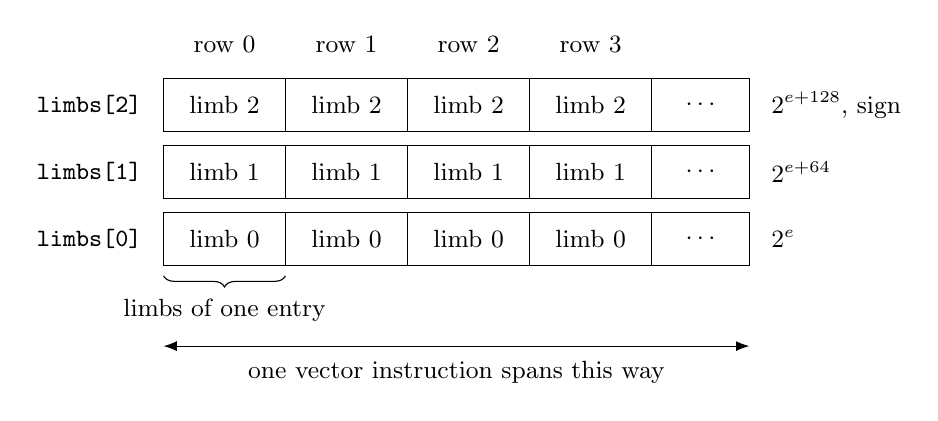
\begin{tikzpicture}[x=1.55cm,y=0.85cm,font=\small]
  \foreach \k/\lab/\sig in {2/limbs[2]/{$2^{e+128}$, sign},1/limbs[1]/{$2^{e+64}$},0/limbs[0]/{$2^{e}$}} {
    \node[anchor=east] at (0,\k) {\code{\lab}};
    \foreach \i in {0,1,2,3} {
      \draw (\i+0.1,\k-0.4) rectangle (\i+1.1,\k+0.4);
      \node at (\i+0.6,\k) {limb \k};
    }
    \draw (4.1,\k-0.4) rectangle (4.9,\k+0.4); \node at (4.5,\k) {$\cdots$};
    \node[anchor=west] at (5.0,\k) {\sig};
  }
  \foreach \i in {0,1,2,3} { \node at (\i+0.6,2.9) {row \i}; }
  \draw[decorate,decoration={brace,mirror,amplitude=4pt}] (0.1,-0.55) -- (1.1,-0.55)
    node[midway,below=5pt] {limbs of one entry};
  \draw[Latex-Latex] (0.1,-1.6) -- (4.9,-1.6) node[midway,below=2pt] {one vector instruction spans this way};
\end{tikzpicture}
\caption{Limb-major storage. Each \code{limbs[k]} is a limb-column: one allocation holding limb $k$ of every row. A vector instruction spans rows; the carry chain of one entry runs down its column of limbs.}
\label{fig:layout}
\end{figure}

Propagating carries along the limbs of a single entry is inherently sequential: limb $k+1$ cannot be computed until after limb $k$. Rows, by contrast, are completely independent of one another, so the limb-major memory layout enables rows to be processed by a single vector instruction (8 64-bit elements at a time on AVX-512), while the sequential carry chain becomes the loop over limb positions, one vector instruction per position.

\section{Per-Column Block Floating Point}

On the assumption that columns contain similarly scaled values, the library implements a block floating-point scheme that shares an exponent per column: not the exponent of its largest value, but the position of the \emph{least significant} bit of any of its values. This arrangement stands in contrast to IEEE standard representations, whose exponents identify the position of the \emph{most} significant set bit. Recall that floating-point values have more than one exact decomposition into an integer times a power of two: 1.0 is exactly $1 \times 2^{0}$, but just as exactly $2^{52} \times 2^{-52}$. IEEE~754 uses the latter, because the most significant set bit is redundant: with the exception of denormals, the format encodes a hidden bit to increase its effective precision. (1.0 is the tidy case, a mantissa of 1 meaning the value is a power of two; nothing about odd normalization reduces every mantissa to a single bit. 3.0 is exactly $3 \times 2^0$, and its 53-bit form is $6755399441055744 \times 2^{-51}$, so \code{frexp} implies a last place fifty-one positions below the value's own rather than fifty-two.)

The power of two specified by a column's exponent, then, is each value's true unit in the last place, or ulp. Taking the minimum over true ulps rather than over standard exponents can save up to 52 bits per column: a column of small integers stays at exponent $2^0$ and one limb wide, whereas a \code{frexp}-based scale would reduce it to $2^{-52}$, forcing the allocation of a second limb holding nothing but zeros. Figure~\ref{fig:entry} shows the bit positions of a three-limb entry.

\begin{figure}[t]
\centering
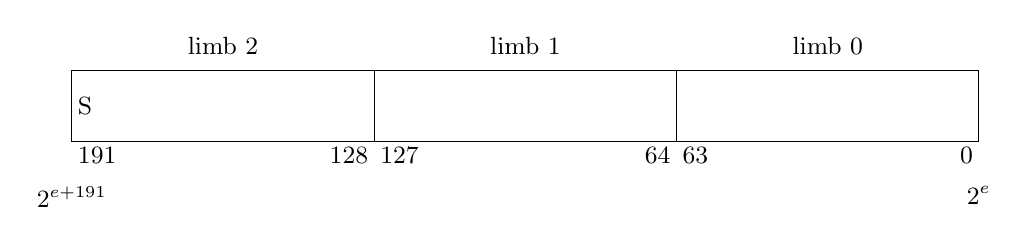
\begin{tikzpicture}[x=0.06cm,y=0.9cm,font=\small]
  % Most significant limb on the left, so each limb runs high bit to low bit.
  \foreach \k/\hi/\lo in {2/191/128,1/127/64,0/63/0} {
    \pgfmathsetmacro{\x}{(2-\k)*64}
    \draw (\x,0) rectangle (\x+64,1);
    \node at (\x+32,1.35) {limb \k};
    \node[anchor=north west,inner sep=2pt] at (\x,0) {\hi};
    \node[anchor=north east,inner sep=2pt] at (\x+64,0) {\lo};
  }
  \node[anchor=west,inner sep=2pt] at (0,0.5) {S};
  \node[anchor=north] at (0,-0.5) {$2^{e+191}$};
  \node[anchor=north] at (192,-0.5) {$2^{e}$};
\end{tikzpicture}
\caption{One entry across three limbs. Bit 0 of limb 0 has significance $2^{e}$, where $e$ is the column's exponent; the top bit of the top limb is the sign.}
\label{fig:entry}
\end{figure}

A column maintains four parameters that must be updated with a survey before applying an accumulation: \code{exponent}, \code{max\_addend\_bits}, \code{add\_count}, and the number of limbs. \code{exponent} can only decrease; the other three only increase. None of them changes on a pre-sized accumulation matrix: when the surveys of every incoming matrix are supplied at construction, \code{exponent} and the limb count are set once from those extents, \code{max\_addend\_bits} and \code{add\_count} are never touched at all, and each accumulate skips the survey, the rescale, and the widen.

\code{max\_addend\_bits} is the greatest number of bits any addend in the column has spanned, counting from the column's current bit 0 up to that addend's most significant bit. \code{max\_addend\_bits} and \code{add\_count}, a running count of the addends, are both updated from a survey of the incoming values, taken before any of those values is added. A rescale adjusts \code{max\_addend\_bits} too, adding the shift it applied, since moving the column's exponent down by that many bits widens every addend's span from the new bit 0 by the same amount. Both exist to bound the width the accumulated sum can reach, so a column whose entries are all zero needs neither. \code{max\_addend\_bits} and \code{add\_count} are cleared when the caller empties the accumulation matrix for reuse, and when a rescale finds every entry already zero, which is also the one case where the exponent can change without shifting anything.

\code{exponent} decreases whenever a value arrives whose least significant set bit sits below the column's current \code{exponent}. Every entry is then left-shifted to match: existing bits move, and none are discarded.

An increase in the limb count, and allocation of one or more new limb-columns, may be prompted by any of three events:
\begin{itemize}
\item a value whose most significant bit sits above the high water mark denoted by \code{max\_addend\_bits};
\item a lower exponent, since that prompts a rescale of \code{shift} bits; and
\item more addends, since a longer run can sum to a larger total.
\end{itemize}

The sum of these considerations determines the number of bits needed for a column:
\begin{equation}
\text{bits} = \code{max\_addend\_bits} + \lceil \log_2(\code{add\_count} + 1) \rceil + 1, \qquad
\text{limbs} = \lceil \text{bits} / 64 \rceil .
\label{eq:width}
\end{equation}
\code{max\_addend\_bits} accounts for the largest single addend; the logarithmic term is headroom reserved above it, gaining one bit each time the count doubles, so that \code{add\_count} addends cannot carry past it; and the final bit is reserved for the sign, which no sum may reach. Rounding the total to the next multiple of 64 gives the number of limbs needed for the allocation.

A batch of input matrices is surveyed before any are accumulated: for any given column, a first pass over the incoming values determines whether the column must be rescaled and widened before any values are added.

Reallocation and rescaling of a column may be prompted by either very large or very small values. Consider a column with 1.0, which sets $\code{exponent} = 0$ and allocates a single limb. Adding a large value to this existing column does not change \code{exponent}, but if more limbs are needed, the newly allocated limbs are initialized with a sign extension (all-zero or all-one copies of the most significant bit of each entry's previous top limb). Adding an extremely small value decreases \code{exponent}, also increases the limb count ($2^{-500}$ drops \code{exponent} to $-500$ and widens the column to 8 limbs; $10^{-300}$ decreases \code{exponent} to $-1049$ and widens the column to 17 limbs), and requires rescaling of the existing limb-columns, left-shifting their contents by exactly the amount \code{exponent} moved and shifting zeros into the least significant bits. Figure~\ref{fig:adjust} contrasts the two adjustments.

\begin{figure}[t]
\centering
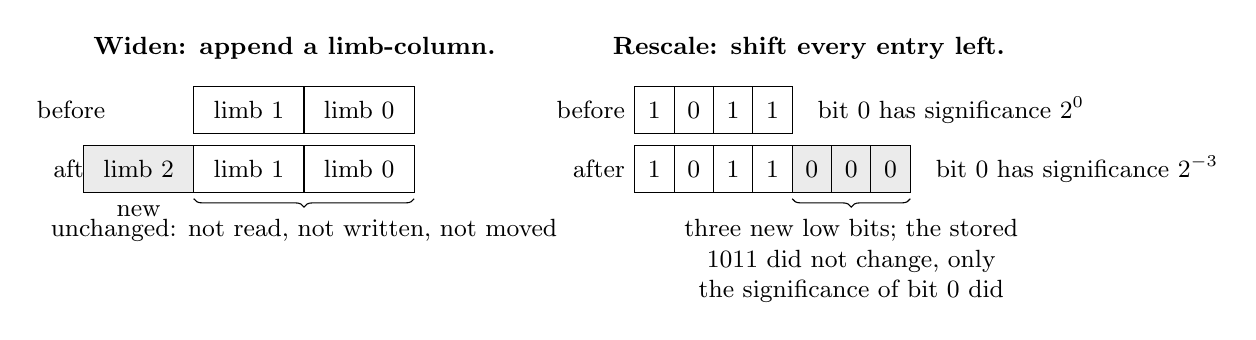
\begin{tikzpicture}[x=1.0cm,y=0.75cm,font=\small]
  % Widen
  \node[anchor=east] at (0,1) {before};
  \draw (1,0.6) rectangle (2.4,1.4); \node at (1.7,1) {limb 1};
  \draw (2.4,0.6) rectangle (3.8,1.4); \node at (3.1,1) {limb 0};
  \node[anchor=east] at (0,0) {after};
  \draw[fill=black!8] (-0.4,-0.4) rectangle (1,0.4); \node at (0.3,0) {limb 2};
  \draw (1,-0.4) rectangle (2.4,0.4); \node at (1.7,0) {limb 1};
  \draw (2.4,-0.4) rectangle (3.8,0.4); \node at (3.1,0) {limb 0};
  \node[anchor=north] at (0.3,-0.45) {new};
  \draw[decorate,decoration={brace,mirror,amplitude=3pt}] (1,-0.5) -- (3.8,-0.5) node[midway,below=4pt] {unchanged: not read, not written, not moved};
  \node[anchor=south west,font=\small\bfseries] at (-0.4,1.7) {Widen: append a limb-column.};
  % Rescale
  \begin{scope}[xshift=6.6cm]
  \node[anchor=south west,font=\small\bfseries] at (-0.4,1.7) {Rescale: shift every entry left.};
  \node[anchor=east] at (0,1) {before};
  \foreach \i/\b in {0/1,1/0,2/1,3/1} { \draw (\i*0.5,0.6) rectangle (\i*0.5+0.5,1.4); \node at (\i*0.5+0.25,1) {\b}; }
  \node[anchor=west] at (2.2,1) {bit 0 has significance $2^{0}$};
  \node[anchor=east] at (0,0) {after};
  \foreach \i/\b in {0/1,1/0,2/1,3/1} { \draw (\i*0.5,-0.4) rectangle (\i*0.5+0.5,0.4); \node at (\i*0.5+0.25,0) {\b}; }
  \foreach \i in {4,5,6} { \draw[fill=black!8] (\i*0.5,-0.4) rectangle (\i*0.5+0.5,0.4); \node at (\i*0.5+0.25,0) {0}; }
  \node[anchor=west] at (3.7,0) {bit 0 has significance $2^{-3}$};
  \draw[decorate,decoration={brace,mirror,amplitude=3pt}] (2,-0.5) -- (3.5,-0.5) node[midway,below=4pt,text width=5.2cm,align=center] {three new low bits; the stored 1011 did not change, only the significance of bit 0 did};
  \end{scope}
\end{tikzpicture}
\caption{The two adjustments. A widen appends a limb-column and leaves every existing limb-column untouched. A rescale lowers the column's exponent and shifts every stored value left by the same amount, so the value each entry denotes is unchanged and nothing is lost.}
\label{fig:adjust}
\end{figure}

A \code{double} arrives as a 53-bit odd mantissa placed at \code{shift}, the distance from its own true ulp down to the column's. Since $53 < 64$, a \code{double} may span at most two limbs, so only \code{off} and $\code{off}+1$ need to be updated, with limbs above $\code{off}+1$ receiving carry propagation until it is absorbed (Figure~\ref{fig:addend}).

\begin{figure}[t]
\centering
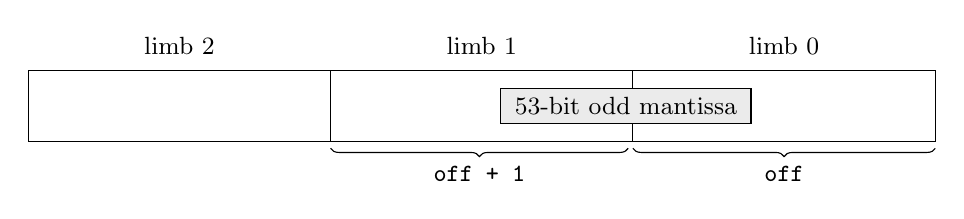
\begin{tikzpicture}[x=0.06cm,y=0.9cm,font=\small]
  \foreach \k in {2,1,0} { \pgfmathsetmacro{\x}{(2-\k)*64} \draw (\x,0) rectangle (\x+64,1); \node at (\x+32,1.35) {limb \k}; }
  \draw[fill=black!8] (100,0.25) rectangle (153,0.75);
  \node at (126.5,0.5) {53-bit odd mantissa};
  \draw[decorate,decoration={brace,mirror,amplitude=3pt}] (128,-0.1) -- (192,-0.1) node[midway,below=3pt] {\code{off}};
  \draw[decorate,decoration={brace,mirror,amplitude=3pt}] (64,-0.1) -- (127,-0.1) node[midway,below=3pt] {\code{off + 1}};
\end{tikzpicture}
\caption{An addend lands in at most two adjacent limbs. Its lowest bit sits \code{shift} positions above the column's bit 0; $\code{off} = \lfloor \code{shift}/64 \rfloor$ selects the lower limb and $\code{shift} \bmod 64$ the bit offset within it.}
\label{fig:addend}
\end{figure}

The carry chain runs fully vectorized, without an overflow test until it reaches the most significant limb, where a sign comparison of the operands is performed against the result.

A column need only allocate as many limb-columns as needed for the dynamic range spanned by its own data. In the bundled demonstration program, a $4 \times 4$ accumulation matrix holding values spanning roughly $10^{-24}$ to $10^{24}$ allocates two and three limbs per column rather than the thirty-three that covering the whole \code{double} range at once would require.

\section{Surveys}

Surveys supply the per-column metadata needed to know how many limb-columns are needed, and whether the column must be rescaled before the survey's matrix is submitted for accumulation.

A survey is 12 bytes per column and contains four fields:
\begin{itemize}
\item \code{min\_exponent}, the lowest true-ulp exponent among the column's nonzero values, taken after normalizing each mantissa to odd rather than from \code{frexp}, so a column of small integers reports 0 and not $-52$;
\item \code{max\_top}, one past the highest bit position any value occupies;
\item \code{any}, true if any value was nonzero;
\item \code{nonfinite}, true if any value was infinite or NaN.
\end{itemize}
Both exponents are \code{int} rather than \code{long long}, since 32-bit exponents can represent six orders of magnitude more range than \code{double} can produce.

Computing a survey requires at most two sweeps over the column (Algorithm~\ref{alg:survey}). The first masks off the sign bit, exits early if any value is infinite or NaN, and computes the maximum of the remaining values, which later is used to compute \code{max\_top}. Additionally, the minimum biased exponent is computed, clamped at 1 so every denormal reports the same one. That minimum is a lower bound on the true ulp: a biased exponent locates the lowest place a significand could occupy, while the true ulp sits above it by the significand's trailing zero count. Unless the column held nothing but zeros, or a non-finite value ended the first sweep, or that bound is larger than a cutoff supplied by the caller, a second sweep of the column is needed to find the significance of each mantissa's least significant set bit and take the minimum in order to compute \code{min\_exponent}.

\begin{algorithm}[t]
\caption{Survey of one column $x_1,\ldots,x_n$ of \code{double}s, given a cutoff $c$}
\label{alg:survey}
\begin{algorithmic}[1]
\State $\mathit{any} \gets \textbf{false}$;\; $\mathit{nonfinite} \gets \textbf{false}$;\; $b \gets +\infty$;\; $m \gets 0$
\ForAll{$x_i$} \Comment{sweep 1: raw bits only}
  \If{$x_i$ is infinite or NaN} $\mathit{nonfinite} \gets \textbf{true}$; \Return \EndIf
  \If{$x_i \ne 0$}
    \State $\mathit{any} \gets \textbf{true}$;\; $b \gets \min(b,\, \max(\mathrm{biased}(x_i), 1) - 1075)$;\; $m \gets \max(m,\, |x_i|)$
  \EndIf
\EndFor
\If{not $\mathit{any}$} \Return \EndIf
\State $\code{max\_top} \gets 1 + \lfloor \log_2 m \rfloor$ \Comment{exact, from the bit pattern of $m$}
\If{$b \ge c$} $\code{min\_exponent} \gets b$; \Return \Comment{no rescale can be due} \EndIf
\State $\code{min\_exponent} \gets +\infty$
\ForAll{$x_i \ne 0$} \Comment{sweep 2: locate the least significant set bit}
  \State $\code{min\_exponent} \gets \min(\code{min\_exponent},\, \mathrm{biased}(x_i) - 1075 + \mathrm{ctz}(\mathrm{significand}(x_i)))$
\EndFor
\end{algorithmic}
\end{algorithm}

An accumulation matrix constructed without surveys computes them itself, one per incoming matrix, and in that case the second sweep is often unnecessary because the accumulation matrix already knows each column's exponent, which it passes as the cutoff. Any incoming value below the column's exponent causes the column to be rescaled; a first-sweep bound at or above the cutoff rules that out on its own. The width does not depend on the second sweep either: \code{max\_addend\_bits} is \code{max\_top} less the column's exponent, and the first sweep computes \code{max\_top} exactly.

A producer computing a survey to send elsewhere has no column to compare against, so the second sweep is always performed. The same is true when the accumulation matrix surveys a column that has no exponent yet: that column will adopt whatever the survey reports, and since a column's exponent only ever moves down, a bound would leave its scale below what its values require, for good.

Functions to update the accumulation matrix include an entry point for a single column, for a column-major matrix, and for a row-major one, which stages each column into contiguous memory. A fourth surveys a matrix already resident on the device, for a producer whose data never touches host memory at all.

Sizing a column from one survey takes its exponent from \code{min\_exponent} and its span from $\code{max\_top} - \code{min\_exponent}$, then adds the headroom of Equation~\ref{eq:width} for however many matrices are coming. Sizing from several surveys of the same column takes the minimum of the minima and the maximum of the maxima. Reducing them to a single aggregate is what makes submission order irrelevant: any matrix inside those extents fits the reservation, so the accumulation matrix never has to know which one is being submitted.

Two adjustments may follow from a survey, one for each extent it reports. A \code{max\_top} above what the column's limb-columns can hold appends more limb-columns, each initialized with a sign extension, and leaves the existing values unchanged. A \code{min\_exponent} below the column's \code{exponent} calls for a rescale: a fresh set of limb-columns is allocated, every stored value is shifted left by the difference with zeros filling the least significant bits, and \code{max\_addend\_bits} is increased by that same shift. The exponent specifies the significance of the lowest bit position the column can hold, so increasing it would right-shift every stored value, dropping bits already accumulated; it only ever decreases. An all-zero column is the exception: \code{max\_addend\_bits} and \code{add\_count} reset to zero, since the total they bound is zero, and the exponent reaches its new value with nothing to reallocate and nothing to shift. It still only decreases, and the number of limb-columns allocated is not changed.

The separation of concerns between matrices and their surveys enables the work to be done by different constituencies (Figure~\ref{fig:datacenter}). In a data center, the nodes that computed the matrices can also compute their surveys and transmit them ahead to the accumulation node; once the accumulation matrix there has been pre-sized to receive them all, the matrices themselves follow, one matrix or even one column at a time. The final output is bit-identical regardless of the order in which they arrive or are processed.

\begin{figure}[t]
\centering
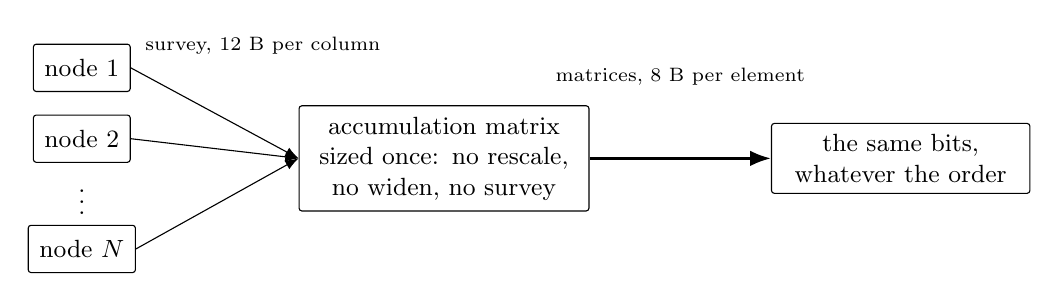
\begin{tikzpicture}[font=\small,
  box/.style={draw,rounded corners=1pt,inner sep=4pt,minimum height=6mm},
  arr/.style={-Latex}]
  % Producers on the left, each sending only its survey.
  \node[box] (n1) at (0,1.5) {node 1};
  \node[box] (n2) at (0,0.6) {node 2};
  \node at (0,-0.1) {$\vdots$};
  \node[box] (nN) at (0,-0.8) {node $N$};
  % The accumulation matrix, sized once from all of them.
  \node[box,text width=34mm,align=center] (acc) at (4.6,0.35)
    {accumulation matrix\\sized once: no rescale,\\no widen, no survey};
  \foreach \s in {n1,n2,nN} { \draw[arr] (\s.east) -- (acc.west); }
  \node[font=\scriptsize,anchor=south] at (2.3,1.55) {survey, 12 B per column};
  % Then the data itself, in any order.
  \node[box,text width=30mm,align=center] (out) at (10.4,0.35)
    {the same bits,\\whatever the order};
  \draw[arr,line width=1pt] (acc.east)
    -- node[font=\scriptsize,above=8mm,midway] {matrices, 8 B per element} (out.west);
\end{tikzpicture}
\caption{Surveys travel ahead of the data. Once the accumulation matrix is sized from all of them, the matrices themselves may arrive and be accumulated in any order.}
\label{fig:datacenter}
\end{figure}

\section{Accumulation}

Since a survey has been performed and applied to the accumulation matrix ahead of time, the accumulation kernel need not concern itself with rescaling or allocation of limb-columns. Every column already has the correct exponent and limb count when the kernel starts, so it can be updated in a single pass over the input (Algorithm~\ref{alg:accumulate}). A value's lowest set bit sits some number of positions above the lowest position the column can hold. That distance, the value's true-ulp exponent minus the column's exponent, is the shift: divided by 64, it gives the limb where the addend starts, and the remainder gives its bit offset within that limb. A 53-bit significand occupies at most two limbs at any bit offset, and the carry propagates upward from the lower limb.

\begin{algorithm}[t]
\caption{Accumulate one column of addends into a column with exponent $e$ and $L$ limbs}
\label{alg:accumulate}
\begin{algorithmic}[1]
\ForAll{rows $i$, eight at a time on AVX-512}
  \State $(m, t, s) \gets$ odd mantissa, true-ulp exponent and sign of $x_i$ \Comment{skip if $x_i = 0$}
  \State $\mathit{shift} \gets t - e$;\; $\mathit{off} \gets \lfloor \mathit{shift}/64 \rfloor$;\; $\mathit{bit} \gets \mathit{shift} \bmod 64$
  \State flag \code{kBadExponent} if $\mathit{shift} < 0$; flag \code{kBadWidth} if the addend's top reaches the sign bit
  \State $a_{\mathit{off}} \gets m \ll \mathit{bit}$;\; $a_{\mathit{off}+1} \gets m \gg (64 - \mathit{bit})$;\; negate the pair if $s$ \Comment{two-limb addend}
  \For{$k = \mathit{off}$ \textbf{to} $L-1$} \Comment{carry chain, one vector op per limb}
    \State $(\code{limbs}[k][i], \mathit{carry}) \gets \code{limbs}[k][i] + a_k + \mathit{carry}$
    \If{$\mathit{carry} = 0$ and $k > \mathit{off}+1$} \textbf{break} \EndIf
  \EndFor
  \State flag \code{kBadOverflow} if the top limb's sign disagrees with both operands'
\EndFor
\end{algorithmic}
\end{algorithm}

A column allocated wide for its dynamic range therefore costs no more per addend than a narrow one, except as required by the input values.

On a pre-sized accumulation matrix, the exponents and limb counts were set at construction from the surveys, which are verified as the accumulation kernel runs: three tests on an addend before it is applied, and a fourth on the running total as it crosses into the top limb.

Between them, those tests detect any deficiencies in the surveys. A survey can understate either of a column's extents, or fail to report a non-finite value; separately, a caller can supply fewer surveys than the matrices it goes on to submit. Each of those throws \code{std::runtime\_error} rather than quietly returning an incorrect sum. They are designed to err on the side of caution: a total that wraps past the sign bit and later wraps back is correct by modular arithmetic, but is reported anyway.

An addend below the column's exponent or too wide for it is skipped; a non-finite one is recorded and applied anyway; and an overflowed sum is left where it wrapped. The rest of the batch goes in either way, and the error is raised afterwards, by which point the accumulation matrix is inconsistent. What it is never left in is a torn state: the kernel loads an entry's limbs, applies whole addends to them, and writes them all back together, so an addend is either absent or present in full.

If no surveys are provided, the accumulation matrix will compute one before beginning the accumulation.

The accumulation matrix only ever touches one column at a time, and accordingly the caller can submit individual columns for accumulation. This interface is useful when matrices are large and columns are much smaller, so only one column and the accumulation matrix have to be resident. A positive or negative power-of-two scale factor may also be specified, and the shift is applied before adding the input into the limb-column.

A symmetric $n \times n$ matrix can be accumulated into one stored triangle. That halves the memory and the input traffic, and the CPU time falls with it, but the deeper reason is exactness. In full storage, the two halves would hold equal values in different limbs under different column scales. Stored once, it cannot drift. The input is assumed to be symmetric.

Accumulation can be spread over worker threads, partitioned by column. Columns are independent in storage and each is touched by exactly one worker, so there is no locking on the hot path and the result is bit-identical to a serial run. Scaling is limited by the CPU's external memory bandwidth.

To conserve bandwidth to the accumulation matrix, batches of input matrices may be accumulated in a single pass: the limbs are read once, every addend applied in registers, and written once.

\section{Reading Back the Result}

Once the accumulation matrix is computed, the library provides the following services.
\begin{itemize}
\item Extraction of its contents at \code{double} precision, correctly rounded: round-to-nearest, ties-to-even, over the full range. \code{to\_double} returns one entry and \code{to\_matrix} the whole thing. A sum beyond the range of a \code{double} reads as $\pm\infty$. One that lands in the denormal range is rounded directly to a multiple of $2^{-1074}$, rather than twice, first to 53 bits and then again on the way into the denormals.
\item Extraction of the \emph{residual}, the portion of each matrix element that rounding dropped, itself correctly rounded. The subtraction is done in the matrix's own fixed point, so the residual is the true difference and not a floating-point estimate of it. It is at most half an ulp of the returned value and is negative exactly when the rounding went up, so the pair is a non-overlapping two-term expansion of about 106 bits. It is $+0.0$ exactly when the value was representable, which \code{is\_exactly\_representable} reports on its own. The residual is optional: \code{to\_double} and \code{to\_matrix} each have an overload that takes somewhere to put it, and the forms without it do no extra work.
\item Extraction of an entry in decimal form by \code{to\_exact\_decimal}, every digit, never rounded. A binary fixed-point value always has a terminating decimal expansion, since $V \cdot 2^{-k} = (V \cdot 5^k)/10^k$, so the expansion is finite however wide the sum. A single 0.1 accumulated once reads back as 0.1000000000000000055511151231257827021181583404541015625.
\item Extraction of the \emph{mean} over a count the caller supplies, correctly rounded as a quotient. Dividing the rounded sum would round twice; \code{to\_double\_mean} and \code{to\_matrix\_mean} round once, by long division of the exact sum, and offer the same residual overloads as the readbacks above. The count is the caller's because the accumulation matrix does not know what a sum stands for: a scaled add is a weighted one, and per-element, per-column and whole-matrix adds all feed the same cell. Neal, whose superaccumulators began as a way to compute the sample mean in R, observes the same double rounding and proposes this single-rounding division as future work~\cite{neal2015}.
\end{itemize}

\section{CUDA Considerations}

When CUDA is available, developers can use \code{CudaAccumulationMatrix}, a separate class that keeps the accumulation matrix in device memory. It is not an acceleration that gets switched on when CUDA is present. Swapping the CPU's scalar kernel for its AVX-512 one leaves the memory and the object identical, so that is a true backend swap and it is chosen at runtime; the CUDA limb arrays are allocated in device memory, and putting them behind the same interface would disguise host-to-device transfers as ordinary calls. What the two implementations share is the algorithm: when to rescale, when to widen, how the exponent moves. The kernels are bandwidth-bound throughout, running at very nearly the card's streaming rate, so performance is determined by how many times an input crosses the bus and how often the CPU and GPU wait on each other.

The constructor for \code{CudaAccumulationMatrix} takes an optional stream parameter which, if specified, is used for every kernel the class launches---the survey, the accumulate, and the sign extension behind a widen and the shift behind a rescale---as well as the stream-ordered allocation and release of the limb-columns and the small copies that bring column extents back to the host and send column descriptors out to the device. Absent a stream, the constructor creates one and destroys it along with the matrix; either way, \code{stream()} returns the one in use. Only a few setup copies stay off the stream, issued synchronously while a column is being allocated or widened, where the ordering they need is already guaranteed.

The survey runs on whichever processor already holds the matrix. A producer holding a matrix in host memory surveys it on the CPU. A producer whose matrix never leaves the device, delivered by GPUDirect or computed there, calls \code{survey\_matrix\_col\_major\_device} instead.

With the extents known before the accumulate launches, the kernel reads each input exactly once, so the input matrix can be read straight out of mapped memory at bus-saturating speeds rather than copying it to device memory first. Input from the host must therefore be page-locked and device-mapped. Input matrices that are not accessible to the accumulation kernel via device memory or mapped pinned memory must be staged to such memory before invoking the kernel.

When reading matrix data from mapped pinned memory, the developer must take care to avoid write-after-read race conditions, since the kernel will still be streaming its input when the call returns. A submission is a kernel launch on the accumulation matrix's stream, so the synchronization may be accomplished by recording a CUDA event on the matrix's stream after updating the matrix. A producer with two buffers in rotation would keep one event per buffer and wait only for the one it is about to refill, never for the stream as a whole.

A producer can avoid the CUDA events altogether by queuing its copies on that same stream, which then orders each copy against the accumulate: a single buffer can be refilled in place, with nothing to wait on. A two-buffer rotation on a caller's stream costs little more per batch than the fill alone, so nearly all of the accumulate hides behind the transfer.

For input matrices in mapped pinned memory, the accumulation runs at bus-saturating bandwidth. Device-resident input is several times faster, and submitting input matrices in batches is faster still, because the limb-columns are read and written once for the whole batch instead of once per matrix.

\section{Performance}

Table~\ref{tab:throughput} reports throughput measured on an 8-core AMD Ryzen 7 7700X and an NVIDIA RTX 3060, in billions of input values accumulated exactly per second. The driver programs that produce these figures are included with the software.

\begin{table}[t]
\caption{Exact accumulation throughput, in $10^9$ input values per second, for column-major inputs of 64 columns. ``Batched $K=8$'' submits eight matrices in one pass over the accumulation matrix.}
\label{tab:throughput}
\begin{tabular}{lrrr}
\toprule
 & $4096 \times 64$ & $16384 \times 64$ & $65536 \times 64$ \\
\midrule
CPU, 1 thread & 0.80 & 0.77 & 0.67 \\
CPU, 8 threads & 4.31 & 4.65 & 1.11 \\
CPU, 8 threads, batched $K=8$ & & & 3.01 \\
GPU, host input & 3.11 & 3.26 & 3.32 \\
GPU, input resident & 4.40 & 6.07 & 8.13 \\
GPU, resident, batched $K=8$ & & & 25.3 \\
\bottomrule
\end{tabular}
\end{table}

Even in elements per second, the figure depends on the values and not only on the shape. A column's width comes from the dynamic range of what is in it, so two matrices of identical dimensions can differ several-fold: values within a few binades of one another share a single limb, while a column reaching across the whole \code{double} range needs thirty-three. Each element costs 8 bytes of input against 16 bytes per limb of accumulation matrix, read and written, so the data sets the width and the width sets the cost. Any single number here describes the inputs it was measured on.

Learning the width has its own cost, and the two adjustments are not alike. Appending a limb-column writes one new array of \code{rows} limbs and reads the one below it to sign-extend from; a rescale allocates a fresh set and moves every limb-column the column already holds. Table~\ref{tab:adjust} shows both on one CPU thread for a $65536 \times 16$ matrix: a submission needing neither ran 1.0\,ms; one appending a limb-column ran 2.0 to 3.0\,ms whatever the column's current width; one forcing a rescale ran 5.0\,ms at two limbs and 12.0\,ms at thirteen, rising with the width because the width is what it rewrites. That asymmetry is why \code{reserve\_for\_surveys} earns its place: a caller who knows roughly how low its data reaches pays for one rescale up front rather than one per submission that reaches lower than the last.

\begin{table}[t]
\caption{Cost of one submission of a $65536 \times 16$ matrix on one CPU thread as the column grows, in milliseconds. Each widen step raises the largest addend by $2^{64}$; each rescale step lowers the smallest by $2^{-64}$. A submission with nothing to adjust costs 1.0\,ms at this shape.}
\label{tab:adjust}
\begin{tabular}{rrr}
\toprule
limbs after & widen & rescale \\
\midrule
2 & 3.0 & 5.0 \\
4 & 2.9 & 5.8 \\
6 & 2.9 & 6.5 \\
8 & 2.7 & 6.8 \\
10 & 2.5 & 8.6 \\
13 & 2.2 & 12.0 \\
\bottomrule
\end{tabular}
\end{table}

On the device the same two adjustments cost differently again, because memory traffic is not what dominates them. Allocating a limb-column from the stream-ordered pool is close to free, at one to two microseconds once the pool has grown to size, against about three milliseconds for the first allocation that grows it. What costs is the synchronization around it. \code{grow\_column} and \code{rescale\_column} each drain the stream before touching the column's array of base pointers, and that array is allocated with plain \code{cudaMalloc} and released with \code{cudaFree}, neither of which is stream-ordered. A widen on the GPU is therefore a pipeline stall rather than a memory pass, taken once per column that needs one, and what it costs is whatever work was in flight when it landed. Pre-sizing removes both calls entirely, which matters more here than on the CPU: the CPU pays a predictable pass over memory, while the device pays for however much work it has to abandon mid-flight.

\section{Software}

The accompanying software component contains the library, its test suite, the demonstration program, the benchmark drivers that produce Tables~\ref{tab:throughput} and~\ref{tab:adjust}, and a user manual describing installation, dependencies and every public entry point. The library is C++17 with no dependencies beyond a C++ compiler and CMake; the AVX-512 kernels are compiled when the compiler supports them and selected at run time, and the CUDA class is built when a CUDA toolkit is found. Future versions of the software package will be made available via~\cite{truesumrepo}.

\section{Conclusion and Future Work}

The accumulation matrix does not offer more precision so much as it removes a variable: no matter which device, or how many cores or threads, or what order data arrives across the network, the same bits are produced every time, because underneath is integer arithmetic in a fixed point wide enough that it never has to round. It bears repeating that exactness is not accuracy. A sum of \code{double}s routinely needs more bits than any one of its addends, which is the whole reason the residual and \code{to\_exact\_decimal} exist, but no amount of exactness recovers information the inputs never held. The fifty-five digits that come back for a single accumulated 0.1 are every one of them correct, and every one of them a fact about the \code{double} nearest 0.1 rather than about the number the caller meant to add.

A survey is twelve bytes per column, small enough to serve as metadata that describes a matrix and enables future accumulations to be sized properly before accumulation begins. Pre-sizing accumulation matrices removes the need to rescale the existing data, or to append limb-columns partway through the accumulation.

Demmel and Nguyen's reproducible sum already began with a pass to find $\max_i |x_i|$, and both they and the ExBLAS authors treated that pass as overhead to be designed away~\cite{demmel2013,iakymchuk2015}. A \truesum{} survey records both extents, the lowest true ulp as well as the highest bit, because an exact sum cannot drop the low bits that a reproducible one rounds away. The node that already holds a matrix can compute its survey and send it ahead of the data. When the accumulation matrix surveys its own input instead, it does so a column at a time, so the accumulate usually finds that column still in cache. Surveys of any number of matrices reduce to one reservation by taking minima and maxima, and a reservation made that way is checked rather than trusted, since the accumulate tests every addend against the extents it was given.

An accumulation matrix holds one accumulator per entry, so the accumulator's size multiplies across every row and column. Ahrens, Demmel and Nguyen show that the memory traffic of a tiled matrix multiply grows with the square root of the accumulator's size, which is why ReproBLAS holds its accumulator to six words and accepts rounding error to do it~\cite{ahrens2016}. Columns sized from their surveys stay small without giving up exactness, to the extent the data allow.

Exact accumulation restores associativity, so whole-matrix, column-major, per-column and per-element accumulation all produce the same output regardless of order of submission; the threaded, batched, symmetric, pre-sized and GPU paths must each match the plain serial one; and the AVX-512 kernels are cross-checked against the scalar ones by forcing the portable path. Catastrophic cancellation ($10^{300} + 1 - 10^{300}$ yields exactly 1), a million values whose ulp is far below the running total, and every rounding tie from $1 + 2^{-53}$ down to the $2^{-1075}$ round-to-zero tie are checked individually. The test suite runs in well under a second and is clean under AddressSanitizer, UndefinedBehaviorSanitizer and ThreadSanitizer.

For future work, several directions suggest themselves.
\begin{itemize}
\item \textbf{Merging two accumulation matrices.} Columns at the same exponent and width add limb-wise with a single carry chain, and columns at different exponents need the rescale the library already performs. A tree reduction requires this operation, and its absence is why the distributed story above ends at sending every matrix to one accumulator rather than combining partial sums pairwise. Every accumulator cited in the introduction already provides one: Kulisch's complete addition, Neal's sum of two superaccumulators, the merge stages of ExBLAS and ReproBLAS's addition of one indexed sum to another. For \truesum{} it is a missing operation, not an open problem.
\item \textbf{Narrower input formats.} \code{float}, \code{half} and \code{bfloat16} all widen to \code{double} exactly, so they need no new kernel, only a conversion at the boundary. The payoff is on the device, where the accumulate is bandwidth-bound and a \code{half} input crosses the bus at a quarter the bytes.
\item \textbf{Exact \code{gemm} through the Ozaki scheme.} Ozaki, Ogita, Oishi and Rump split $A$ by rows and $B$ by columns into slices narrow enough that the product of any two slices, computed by an ordinary \code{gemm}, is exact, which turns $AB$ into an unevaluated sum of floating-point matrices~\cite{ozaki2012}. Their paper leaves that sum to an accurate summation algorithm and stores every product matrix until then, which the authors call a drawback: working space significantly larger than \code{gemm}'s. An accumulation matrix can take each product as it is formed and sum all of them exactly, with no change to its kernels, since every addend is an ordinary \code{double}. The surveys come from the splitting itself. Every entry of a slice product is an integer multiple of $u^2 \sigma_i \tau_j$ and at most $u \sigma_i \tau_j$ in magnitude, where $u$ is the unit roundoff and $\sigma_i$ and $\tau_j$ are the powers of two the splitting already chose for row $i$ of $A$ and column $j$ of $B$, so each product can be submitted pre-sized and checked as it accumulates, provided no slice product underflows, which the scheme assumes as well. The scheme needs more slices as the dynamic range within a row or column grows, just as a \truesum{} column needs more limbs.
\item \textbf{Exact products without splitting.} The product of two \code{double}s is exact in 106 bits, which a fixed-point accumulator holds without rounding, so an exact dot product can also be built by widening the addend instead. The products are formed on the fly, so none exists ahead of time to survey, but a product's extents are bounded by its factors': its true ulp is exactly the sum of theirs, and its top at most the sum of their tops, so the surveys of the two input matrices are enough to size the accumulation. The exponent range doubles with it, so the worst case grows accordingly.
\item \textbf{A spill path for wide batches.} The AVX-512 batch kernel holds a row's limbs in registers, capping the batch at eight limbs; wider columns fall back to one matrix at a time and give up the batching saving exactly where columns are widest and it would be worth most.
\item \textbf{binary128.} Every format above is narrower than \code{double} and rides the existing path. A wider one does not: 113 bits of significand breaks the two-limb placement that all three kernels are built around.
\end{itemize}

\begin{acks}
Claude (Anthropic), used through Claude Code, assisted in preparing this work: it drafted and revised sections of the text under the author's direction, wrote and ran the benchmark programs whose measurements appear in Tables~\ref{tab:throughput} and~\ref{tab:adjust}, located and summarized several of the cited works, and contributed to the library's source code. The author reviewed all generated material, verified the citations against their sources, and is responsible for the content.
\end{acks}

\bibliographystyle{ACM-Reference-Format}
\bibliography{truesum}

\end{document}
